\chapter{Introduction}\label{introduction}

Generally, machine learning applications build models depending on training data which is gathered collectively by using a specific data acquisition tool. This process introduces a number of problems regardless of quality and amount of the gathered training data. First of all, the data acquisition process itself can cost lots of time and money since the data has to be labelled by human workers. Moreover if the domain in which the training data is collected from is very specific, for example medical text, certain number of domain experts might be needed. In the cases where the domain experts cannot be employed, gathering necessary amount of data to build a model can be impractical or impossible. Secondly, training on previously gathered large datasets with traditional supervised learning can be very computationally expensive. Thirdly and most importantly, data distribution of the domain where the target application operates can change which leads to existing training data to become outdated. Since the model is not trained with the changed data coming from the environment, it performs poorly. This phenomenon is called concept drift in the literature \cite{concept}. In this case more training data has to be gathered and the model has to be re-trained with the new data, both of which can be again impractical or impossible depending on the resources at hand.

These mentioned problems make us to think about a data acquisition process where the training data is collected interactively and iteratively with a model which adapts to the continuous data stream. In the proposed design, the model is trained continuously with each iteration of data acquisition process instead of training by traditional supervised learning with large amount of data. The model not only aims to automatically adapt to new training data without any retraining from scratch, it also interacts with human users by providing suggestions to users and making use of user feedback as a form of input to train. With this human-in-the-loop paradigm, necessity of collecting a large dataset in advance is eliminated and a functional model (even though it is not fully optimal to use) is created very fast, at the same time. This paradigm is called adaptive learning. Figure 1.1 shows the basic workflow of suggested data acquisition process. The goal is to create a model which has comparable or better performance than a model trained with traditional supervised learning at the end of data acquisition process. Figure 1.2 shows a real world human-in-the-loop data acquisition system for text simplification.

\begin{figure}[h]
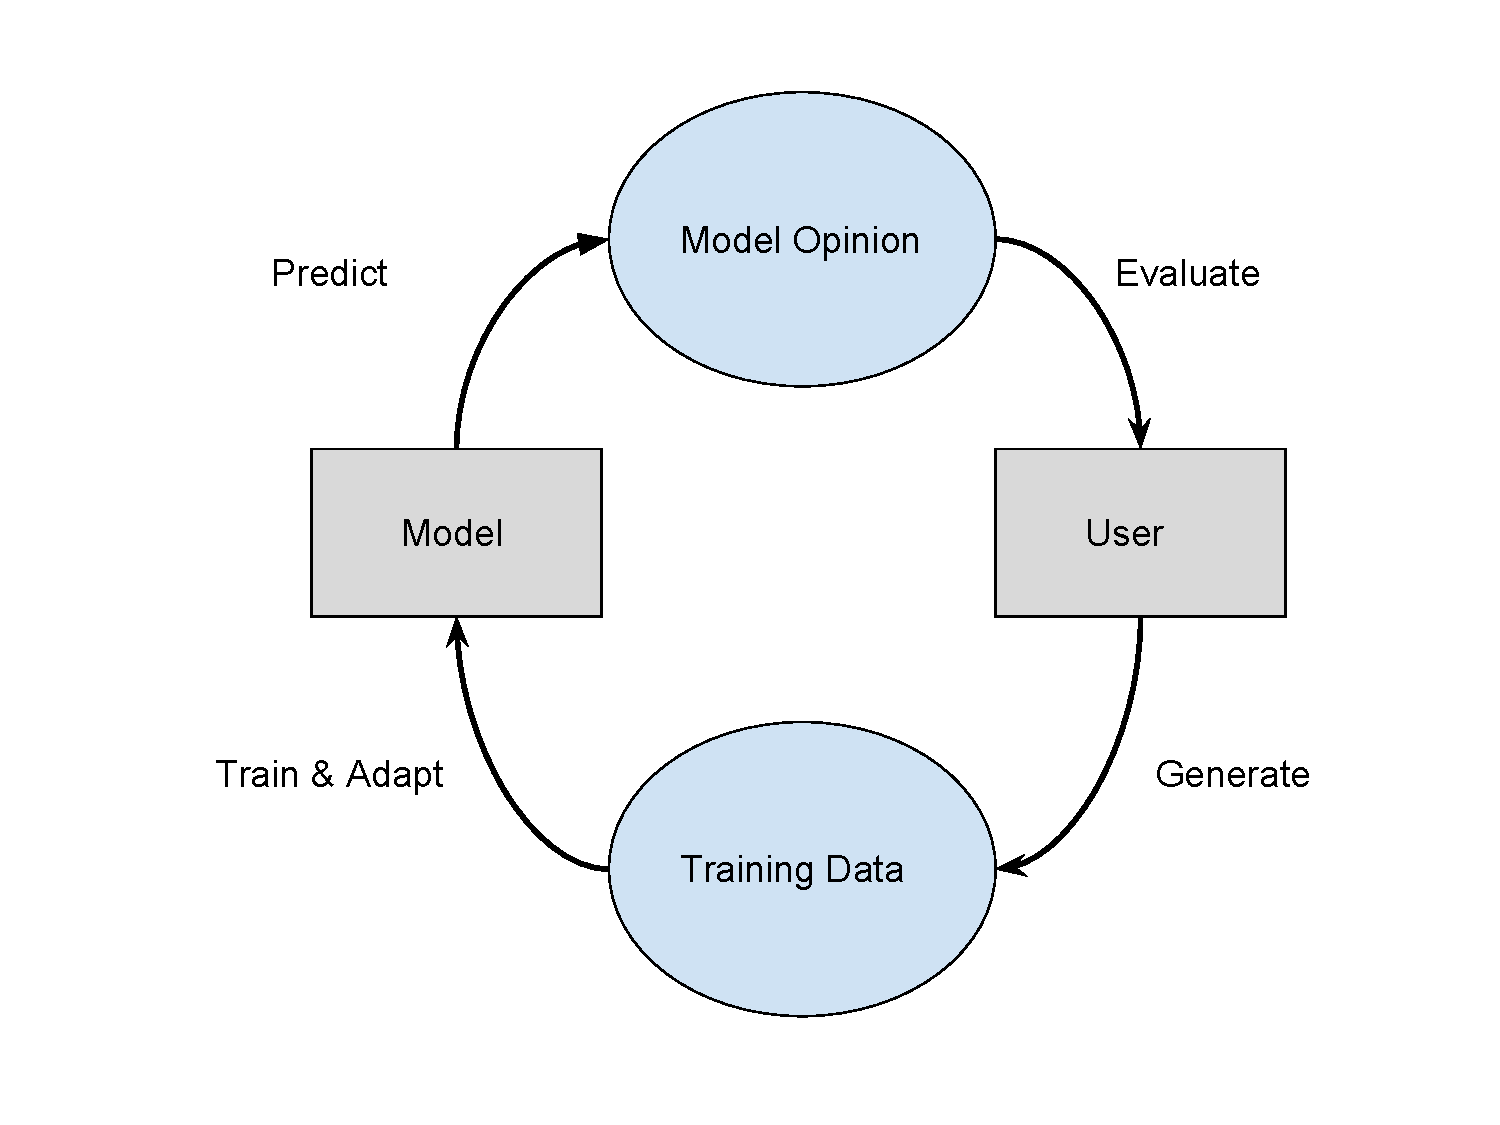
\includegraphics[width=\textwidth, height=10cm]{hil}
\centering
\caption{Human in the loop data acquisition.}
\end{figure}

Main focus of this thesis is the behaviour of deep neural models in human-in-the-loop settings which is described above. Different learning strategies for training deep neural models are studied and experiments with different training methods are conducted in order to investigate their effectiveness in continuous data streams. Additional learning strategies are also proposed in order to overcome some of the problems which are introduced by human-in-the-loop setting. Although human-in-the-loop data acquisition can help with the problems which are described in the beginning of this section, it also introduces some other problems in the context of modelling. As a starting point, it is shown that a deep neural model in fact can adapt and improve with the continuously increasing data and then different learning strategies are studied, each of which addressing a different problem in human-in-the-loop setting. Instead of traditional supervised learning, incremental learning is studied in order to obtain adaptivity to incoming data without forgetting previous knowledge. Learning strategies that are proposed, are mainly concerned with how the model processes the incoming data. 

Incremental learning is shown to be able to create a relatively good and usable model, way before the model is exposed to all of the training data. Experiments with transfer learning are done in order to simulate a concept drift scenario where a general model comes across to new training data with different nature. With the same experiments, a situation in which the system does not have enough resources to collect significant amount of data, is also simulated. It is also shown that with transfer learning, it is possible to create a model which is impossible to create with the available data. Additionally, different active learning strategies are studied in order to reduce the data we need to build a satisfactory model.  At the end, experiments in which these strategies are combined together are done and their results are reported.

\begin{figure}[h]
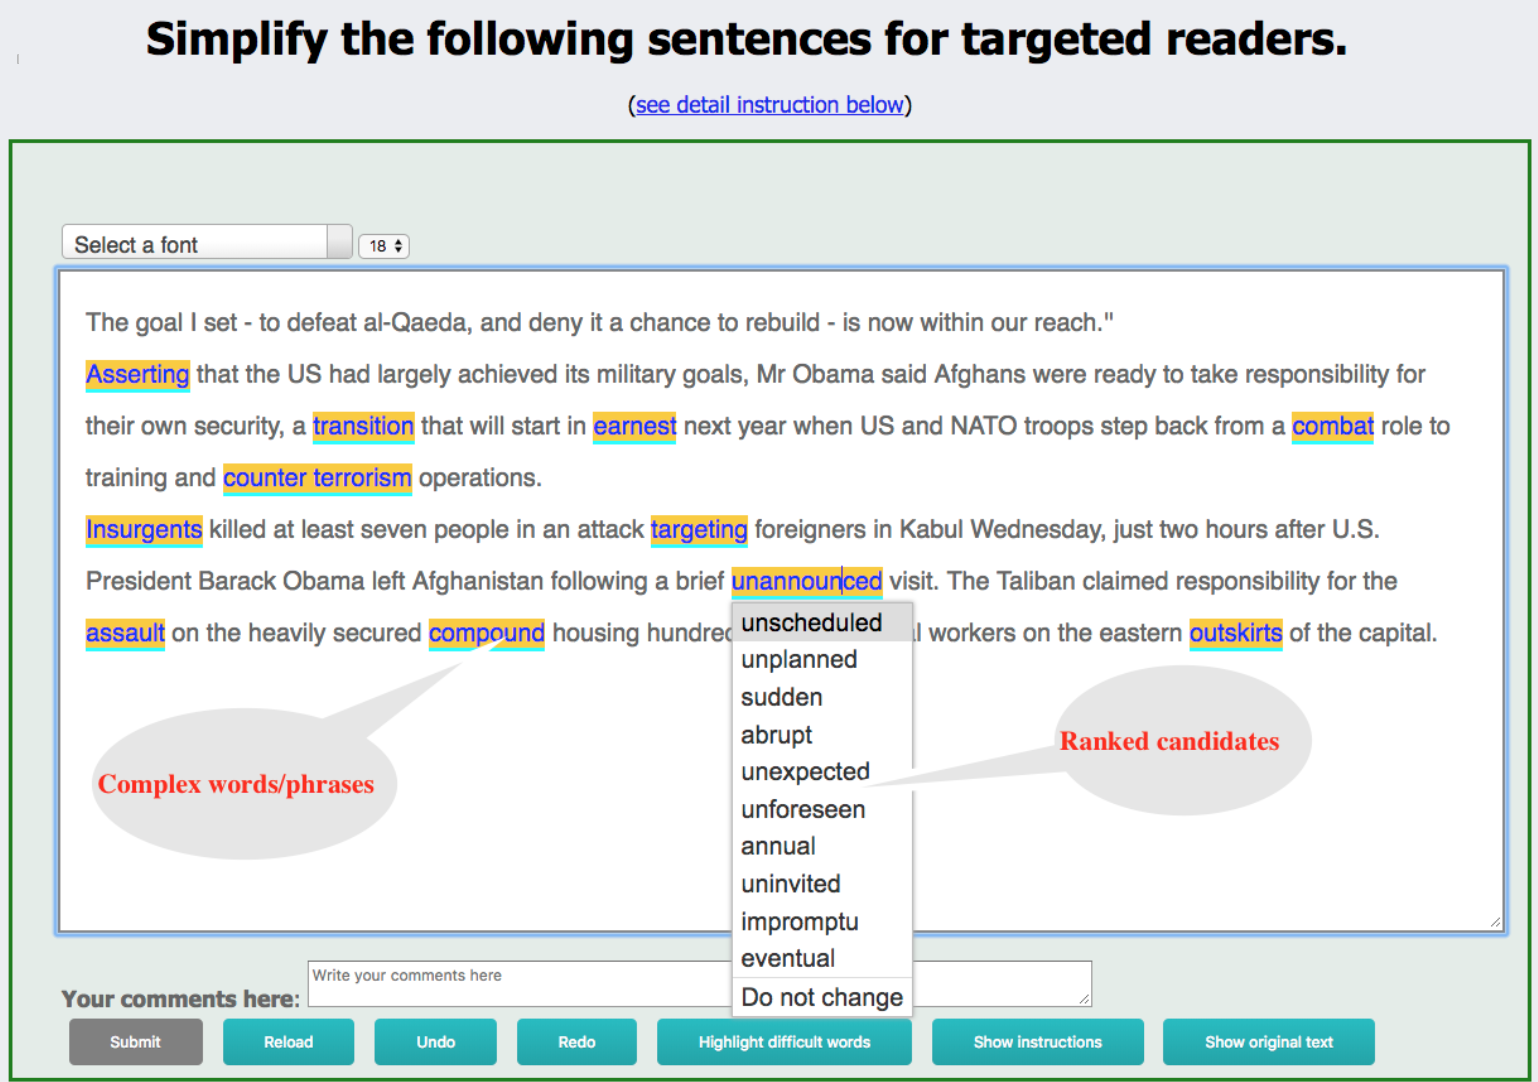
\includegraphics[width=\textwidth]{human-in-the-loop}
\centering
\caption{An interactive human-in-the-loop application for text simplification \cite{par4sim}. Target words to be simplified are highlighted and user is provided with a list of candidate words to choose from. Candidate words are generated and ranked by the system/model.}
\end{figure}


Paraphrase generation is chosen as the target application. Paraphrase generation is the problem of generating different texts from a source text while retaining the meaning. It has various application areas in Natural Language Processing (NLP) like dialogue systems where it is used for building more natural conversional agents, information retrieval where it is used for enhancing retrieval process, natural language generation where it is used for generating training data for different NLP tasks and text summarization where it is used for replacing a text with a simpler paraphrase of it. Generating the text "President Trump strongly denied any wrong doing in this matter." from the text "POTUS firmly denied any fault in this subject." would be a good example of paraphrase generation. It is a challenging problem because of many different reasons. There are more than one way to paraphrase a source sentence and the quality of generated paraphrase depends on many things like context information, lexical and semantic diversity and so on. Therefore the problem is not only concerned with language generation, it also deals with language understanding. Another problem which is introduced by picking paraphrase generation as our target application is out of vocabulary words. 

Deep neural models for NLP problems is built on predefined and specific vocabularies which are usually constructed from training data. These vocabularies cannot be changed or expanded during or after training. Since the model does not know the words which it have not seen in the training, unknown words can lead to poor performance. This is an open problem in NLP and all neural models suffer from it but in our case it is more problematic because of the setting which is studied and nature of the problem. In our setting data comes to the system continuously and the model is trained continuously therefore adapting model strictly depends on the vocabulary which it started training with. Additionally paraphrase generation is not a classification or regression task, it is a generation task therefore we do not know target texts (paraphrases) for our source texts beforehand, they are generated by users. These two mentioned reasons cause our model to be more prone to out of vocabulary words since there will be more of them compared to traditional supervised setting. There are two possible solutions for this problem. First solution is to use pre-trained word embeddings for our neural net instead of training our own word embeddings. These pre-trained word embeddings are built on very large corpuses so they would cover a lot of out of vocabulary words for our training data. Second solution is to design a data acquisition process similar to \cite{par4sim} where the system suggests paraphrase candidates which are created from large, existing resources and make the user choose from suggestions. Even though this puts restrictions to the users, it ensures that the target paraphrases are built from a known vocabulary. Since the vocabulary is known beforehand the model can train its own word embeddings. In this thesis the latter solution is simulated. 

The human-in-the-loop process described in this section is simulated by dividing a large existing dataset into subsets and feed the model with these subsets iteratively. In each iteration, the model gets a new batch of data and updates itself according to it. The model is trained with these batches using different learning strategies and evaluate it on a separate test set at the end of each iteration, observing the model's behaviour through time.

According to our knowledge there is no work studying neural paraphrase generation in human-in-the-loop settings especially concerning adaptivity of the neural model. Moreover this work seems to be first to try incremental learning and active learning for neural paraphrase generation. This thesis also builds on to existing transfer learning research for neural paraphrase generation by experimenting with different methods of transfer and analysing the transfer process.

\section{Thesis Organization}
This thesis is organized as follows; the rest of this chapter provides the research questions that are investigated and a review of state-of-the-art works in neural paraphrase generation, human-in-the-loop learning and the learning strategies used in this work. In Chapter 2, the main methodology and technical details regarding our deep neural model are explained which are followed by the description of main ideas behind the learning strategies. Chapter 3 describes the details of the learning strategies, the datasets and evaluation metric used in this work. It also explains the experimental setups in detail with their corresponding reasonings. In Chapter 4, results of the experiments are presented, the findings are explained and a discussion on the overall findings of the thesis is provided. The two last chapters give the conclusion and an extensive list of future work.

\section{Research Questions}

This thesis is going to aim to investigate whether deep neural models can be combined with adaptive learning, human-in-the-loop paradigm for paraphrase generation task. The basic research questions can be summarized as below:

\begin{itemize}
  \item Can deep neural models effectively adapt and gradually perform in a continuous data stream for paraphrase generation?

Considering the fact the deep neural models need a lot of training data to perform well, is it possible to integrate this type of models into human-in-the-loop setting? The model is expected to learn and adapt continuously since retraining large models over and over again through time, is not desirable. The main goal is to determine whether such models can be applied to real world applications which have similar setting to ours. If the answer is yes, what should be the training scheme (how to make use of incoming data stream) for such models? Basically we would like to know if continuous learning is possible for neural paraphrase generation. 
 
  \item Can the model achieve better or comparable performance than traditional supervised learning by leveraging the data stream?
  
  Can adaptive learning improve accuracy by adding more generalization power? Can the model achieve better or comparable performance with less data? It is also possible that training a deep neural network in adaptive manner may have a negative effect, if so it will be insightful to understand the reason why. Understanding how deep models behave under this training paradigm is an interesting and challenging question.
   
  \item What are the possible challenges/limitations introduced by system and model in this setting and what are the possible learning strategies that can be used for dealing with these challenges?
  
  It is important to determine what kind of existing learning strategies that can used to perform better in human-in-the-loop setting. This is particularly important since the setting itself imposes some challenges. How can the model deal with challenges like limited resources and concept drift? Additionally training deep neural models continuously introduces challenges of its own like overfitting and underfitting depending on the training data.

\end{itemize}

Considering the lack of research in this area, with these questions answered, it might be possible to enhance the performance of deep neural models (shorter training time and / or better paraphrases) in paraphrase generation task and create a framework on adaptive learning for future research.

\section{Related Work}

Deep learning based approaches have been quite successful in various NLP tasks including language modelling \cite{siriam}, automatic speech recognition \cite{hannun} and neural machine translation \cite{cho}. Main idea behind deep learning is learning future representations of the dataset instead of depending on hand crafted features engineered by domain experts. Deep neural models is capable of hidden representations and relationships inside the data which are not possible to obtain by feature engineering. In the case of NLP, deep neural models are capable of capturing lexical, semantical and contextual relationships between textual data points which makes them quite successful. Nowadays, almost all of the state-of-the-art models used in NLP applications are based on deep learning.

For the task of paraphrase generation, deep learning is already proved to be extremely successful by the work which has been done in past few years. Especially with the development of sequence to sequence learning \cite{Vinyalsetal}, a lot of research has been emerged, building models for paraphrase generation using this framework. \cite{Prakashetal} introduces a sequence to sequence model based on stacked LSTM's with residual connections. The authors use residual connections between stacked LSTM networks in order to address exploding/vanishing gradient problems for LSTM based models. They have experimented on different large scale datasets to show the effectiveness of their model which can produce meaningful, semantically and grammatically correct paraphrases. They also show that with residual connections, the LSTM based model can learn how to retain important words better. A lightweight variant of this model is used in this thesis.

\cite{Guptaetal} uses deep generative models coupled with LSTM's in sequence to sequence framework, in order to generate paraphrases. They modify the model by conditioning generative model with source sentence in order to enhance performance. They have managed to outperform state-of-the-art methods for paraphrase generation and generate a baseline for Quora Question Pair dataset which we use in this thesis. Additionally they evaluate their model with human evaluation which suggest the model can create good and relevant paraphrases. This work is particularly interesting since the resulting model can also link unseen concepts which are related to the original sentences.

\cite{Lietal} uses a very interesting approach, using recently popularized deep reinforcement learning for paraphrase generation. Their approach uses two components, a generator which is a sequence to sequence model, responsible for creating paraphrases, and an evaluator which is a deep matching model, responsible for recognizing paraphrases. Main idea is the evaluator enhancing the performance of generator. They propose this framework as a solution for lack of evaluation metrics for paraphrase generation. Their approach outperforms the state-of-the-art methods in paraphrase generation in both human evaluation and automatic evaluation.

Interactive data acquisition tools for NLP tasks has been worked on quite extensively in recent years. Many different tools are designed and implemented in order to enhance the ability to collect and use complex text data. They make use of multiple visualizations, correction mechanisms and machine learning based feedback loops. \cite{trivedi} developed an interactive user interface for enabling NLP tasks on clinical text which requires domain expertise. \cite{Yimam:2016aa} developed a tool for applying interactive, human-in-the-loop machine learning to biomedical entity and relation recognition. They demonstrate the effectiveness of their approach by simulating human-in-the-loop data acquisition with three experiments and prove their concept for adaptive learning. Following this work, \cite{par4sim} creates an adaptive learning system for text simplification which is integrated with a machine learning model. The system effectively makes use of the model in the data acquisition process, creating a feedback loop with human workers. They have done a real-time data acquisition using the Amazon MTurk crowdsourcing platform. They showed successful integration of their model and its adaptiveness through time by evaluating the model's performance and showing its improvement over time. This thesis is inspired by this particular work, replaces the model used with a deep neural model and studies its behaviour. For the adaptive, continual learning in neural networks \cite{parisi} gives an extensive review on the subject, covering different number of techniques (some of them are utilized in this thesis) to achieve adaptive learning. In this thesis, adaptive learning is studied in the context of both applicability in real world and learning capability.

In case of transfer learning, it has been already established that knowledge transfer is possible and quite effective in computer vision. Recently, there has been substantial work on its possible applicability on the field of NLP also. An extensive look on knowledge transfer on different NLP tasks is provided in \cite{mou}. They do systematic experiments on different NLP problems to determine what kind of aspects of natural language and network layers are transferable. They show that knowledge transfer is possible between different datasets of same task and semantically similar tasks even though improvement from transfer learning depends on the datasets and the tasks at hand. \cite{zoph} successfully applies transfer learning to neural machine translation, gaining significant increase in performance for translation of low-resource languages. \cite{brad} uses transfer learning for neural paraphrase generation, effectively boosting the performance. Even though they successfully show that knowledge transfer is possible for neural paraphrase generation they do not study different ways to transfer. In this thesis, a layer-by-layer analysis is conducted for studying the performance of different transfer methods and what part of the network is being transferred. Finally, \cite{yoon} studies different transfer schemes for creating personalized language model from a general model. Building on these previous works, a detailed investigation of transfer learning in neural paraphrase generation, is provided.

For active learning, as far as our knowledge is concerned there is no previous work done for paraphrase generation. \cite{shen} successfully applies active learning for name entity recognition based on different sampling strategies. \cite{zhao} uses a sampling strategy based on a combination of model uncertainty and representativeness of data points, applying it on short-text classification. \cite{rubio} successfully applies it on interactive machine translation. Even though it has never been applied on paraphrase generation, these works show that active learning can be used for a variety of NLP tasks. In this thesis, some of the sampling strategies that are proposed in these works, are applied to paraphrase generation.